\section{Benchmark and Experimental Setup}
\label{sec:setup}

\subsection{Tasks}
We build directly on \textsc{ParEval}~\cite{pareval}, the standard benchmark for
LLM-generated parallel code, reusing its function-completion prompts, its
randomized-input drivers, and---crucially---its \emph{serial reference}
implementations as our trusted oracle $R_t$. We draw the OpenMP tasks whose
correct result is sensitive to how the work is parallelized: histograms
(shared-bin updates), reductions (associativity and commutativity of the
combine), scans (loop-carried dependence), and searches (order-dependent
selection). These instantiate the hazard classes of Table~\ref{tab:hazards}. Each
prompt states the required computation and signature but never dictates the
parallelization strategy, so the model must choose a race-free, order-correct
implementation on its own.

\subsection{Oracle and Data}
Correctness is adjudicated by \textsc{ParEval}'s own driver: for each generated
completion the driver compiles the model's function together with the serial
reference, generates randomized inputs, runs both, and reports whether their
outputs agree. Using the benchmark's serial reference as the oracle means the
ground truth is independent of the parallel implementation under test, and the
randomized multi-input validation prevents a program from passing on a single
lucky example. Because the oracle is a sequential program, it is itself immune to
the parallel hazards we study.

\subsection{Differential Verifier and Configurations}
The novel component of our harness is a \emph{distribution-aware differential
verifier}. Rather than validating a completion once, it compiles the program with
OpenMP and executes it across a thread-count sweep $\tau\in\{1,2,4,8\}$ with
repeated runs at each setting, checking every run against the serial reference. A
program is robustly correct only if it validates at every thread count and every
repetition (Eq.~\ref{eq:R}); a result that changes with the thread count, or that
varies across repetitions at a fixed thread count, is the signature of a data
race or an order-dependent computation and is reported as \emph{not robust} with a
diagnostic. Repeated execution is what lets the verifier catch nondeterministic
races that a single validation---\textsc{ParEval}'s default, and an ordinary
agent's execute-and-fix signal---can miss. Compilation and execution run on a
dedicated multi-core cloud VM; the verifier, prompts, and per-run transcripts are
released for reproduction in line with the SC26 reproducibility initiative.

\subsection{Model Panel}
We evaluate \Nmodels{} state-of-the-art instruction-tuned models from a single
provider, spanning a current frontier general-purpose model, its preceding
generation, a code-specialized model, and a higher-reasoning ``pro'' variant---all
accessed through Azure AI Foundry under Entra ID authentication, with no API keys
stored. Holding the benchmark, harness, and prompts fixed, this within-provider
panel spans capability and specialization tiers while controlling for
provider-specific idiom: a tool effect---or its absence---that holds across all
\Nmodels{}, including a model tuned specifically for code, is unlikely to be an
artifact of a single weak or idiosyncratic model. Our harness is model-agnostic and
reaches any deployment through one uniform API. We exploit this to add an
\emph{open-weights} panel---\NopenModels{} models served through an
OpenAI-compatible gateway on a research cluster, spanning a 120B general model and a
27B model---which we run on the race-prone task subset to probe the
capability-dependence of the verifier's value (Section~\ref{sec:crosscap}); a
broader cross-vendor sweep remains future work (Section~\ref{sec:discussion}).
Generation in the baseline condition
is single-shot with no tool use: the model receives the prompt and returns a
completion, which the harness compiles and verifies as-is. Every
generation---system prompt, user prompt, raw response, extracted code, and
verifier feedback---is logged as a reusable artifact.

\subsection{Agentic Tool-Ablation Setup}
For the tool-ablation (Section~\ref{sec:agent}) we run the same
propose--observe--repair agent at levels L0 (single-shot), L1 (execute-once), and
L2 (differential verify), holding the model, prompt, and repair budget $B$ fixed
and varying only the verification tool (Fig.~\ref{fig:pipeline}). The agent completes the task, the tool
returns an observation, and---for L1 and L2---the agent repairs on failure until
the tool reports success or the budget is exhausted. Regardless of condition, the
\emph{final} program of every run is scored by the full differential verifier over
the complete thread sweep, an outcome measure independent of which tool the agent
was permitted to use. Every repair round---the verifier feedback and the revised
program---is logged, so the agent's tool-use and repair trajectory is fully
auditable.

\begin{figure}[t]
\centering
\IfFileExists{../results/figures/fig_pipeline.pdf}
  {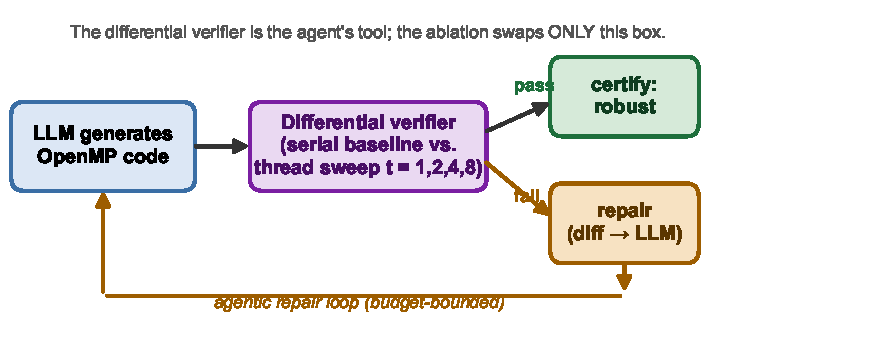
\includegraphics[width=0.99\linewidth]{../results/figures/fig_pipeline.pdf}}
  {\fbox{\parbox{0.8\linewidth}{\centering\vspace{2em}\textsc{[pipeline schematic]}\vspace{2em}}}}
\caption{The agentic pipeline. The model proposes a completion; the tool returns an
observation (nothing at L0, a single-thread pass/fail at L1, or the full
thread-sweep verdict at L2); on failure the agent repairs until the tool reports
success or the budget is spent. Every run's \emph{final} program is scored by the
full differential verifier, independent of the tool the agent could use.}
\label{fig:pipeline}
\end{figure}
